
\section{Proposed Method}

\subsection{Overall Architecture}

\begin{figure*}
    \centering
    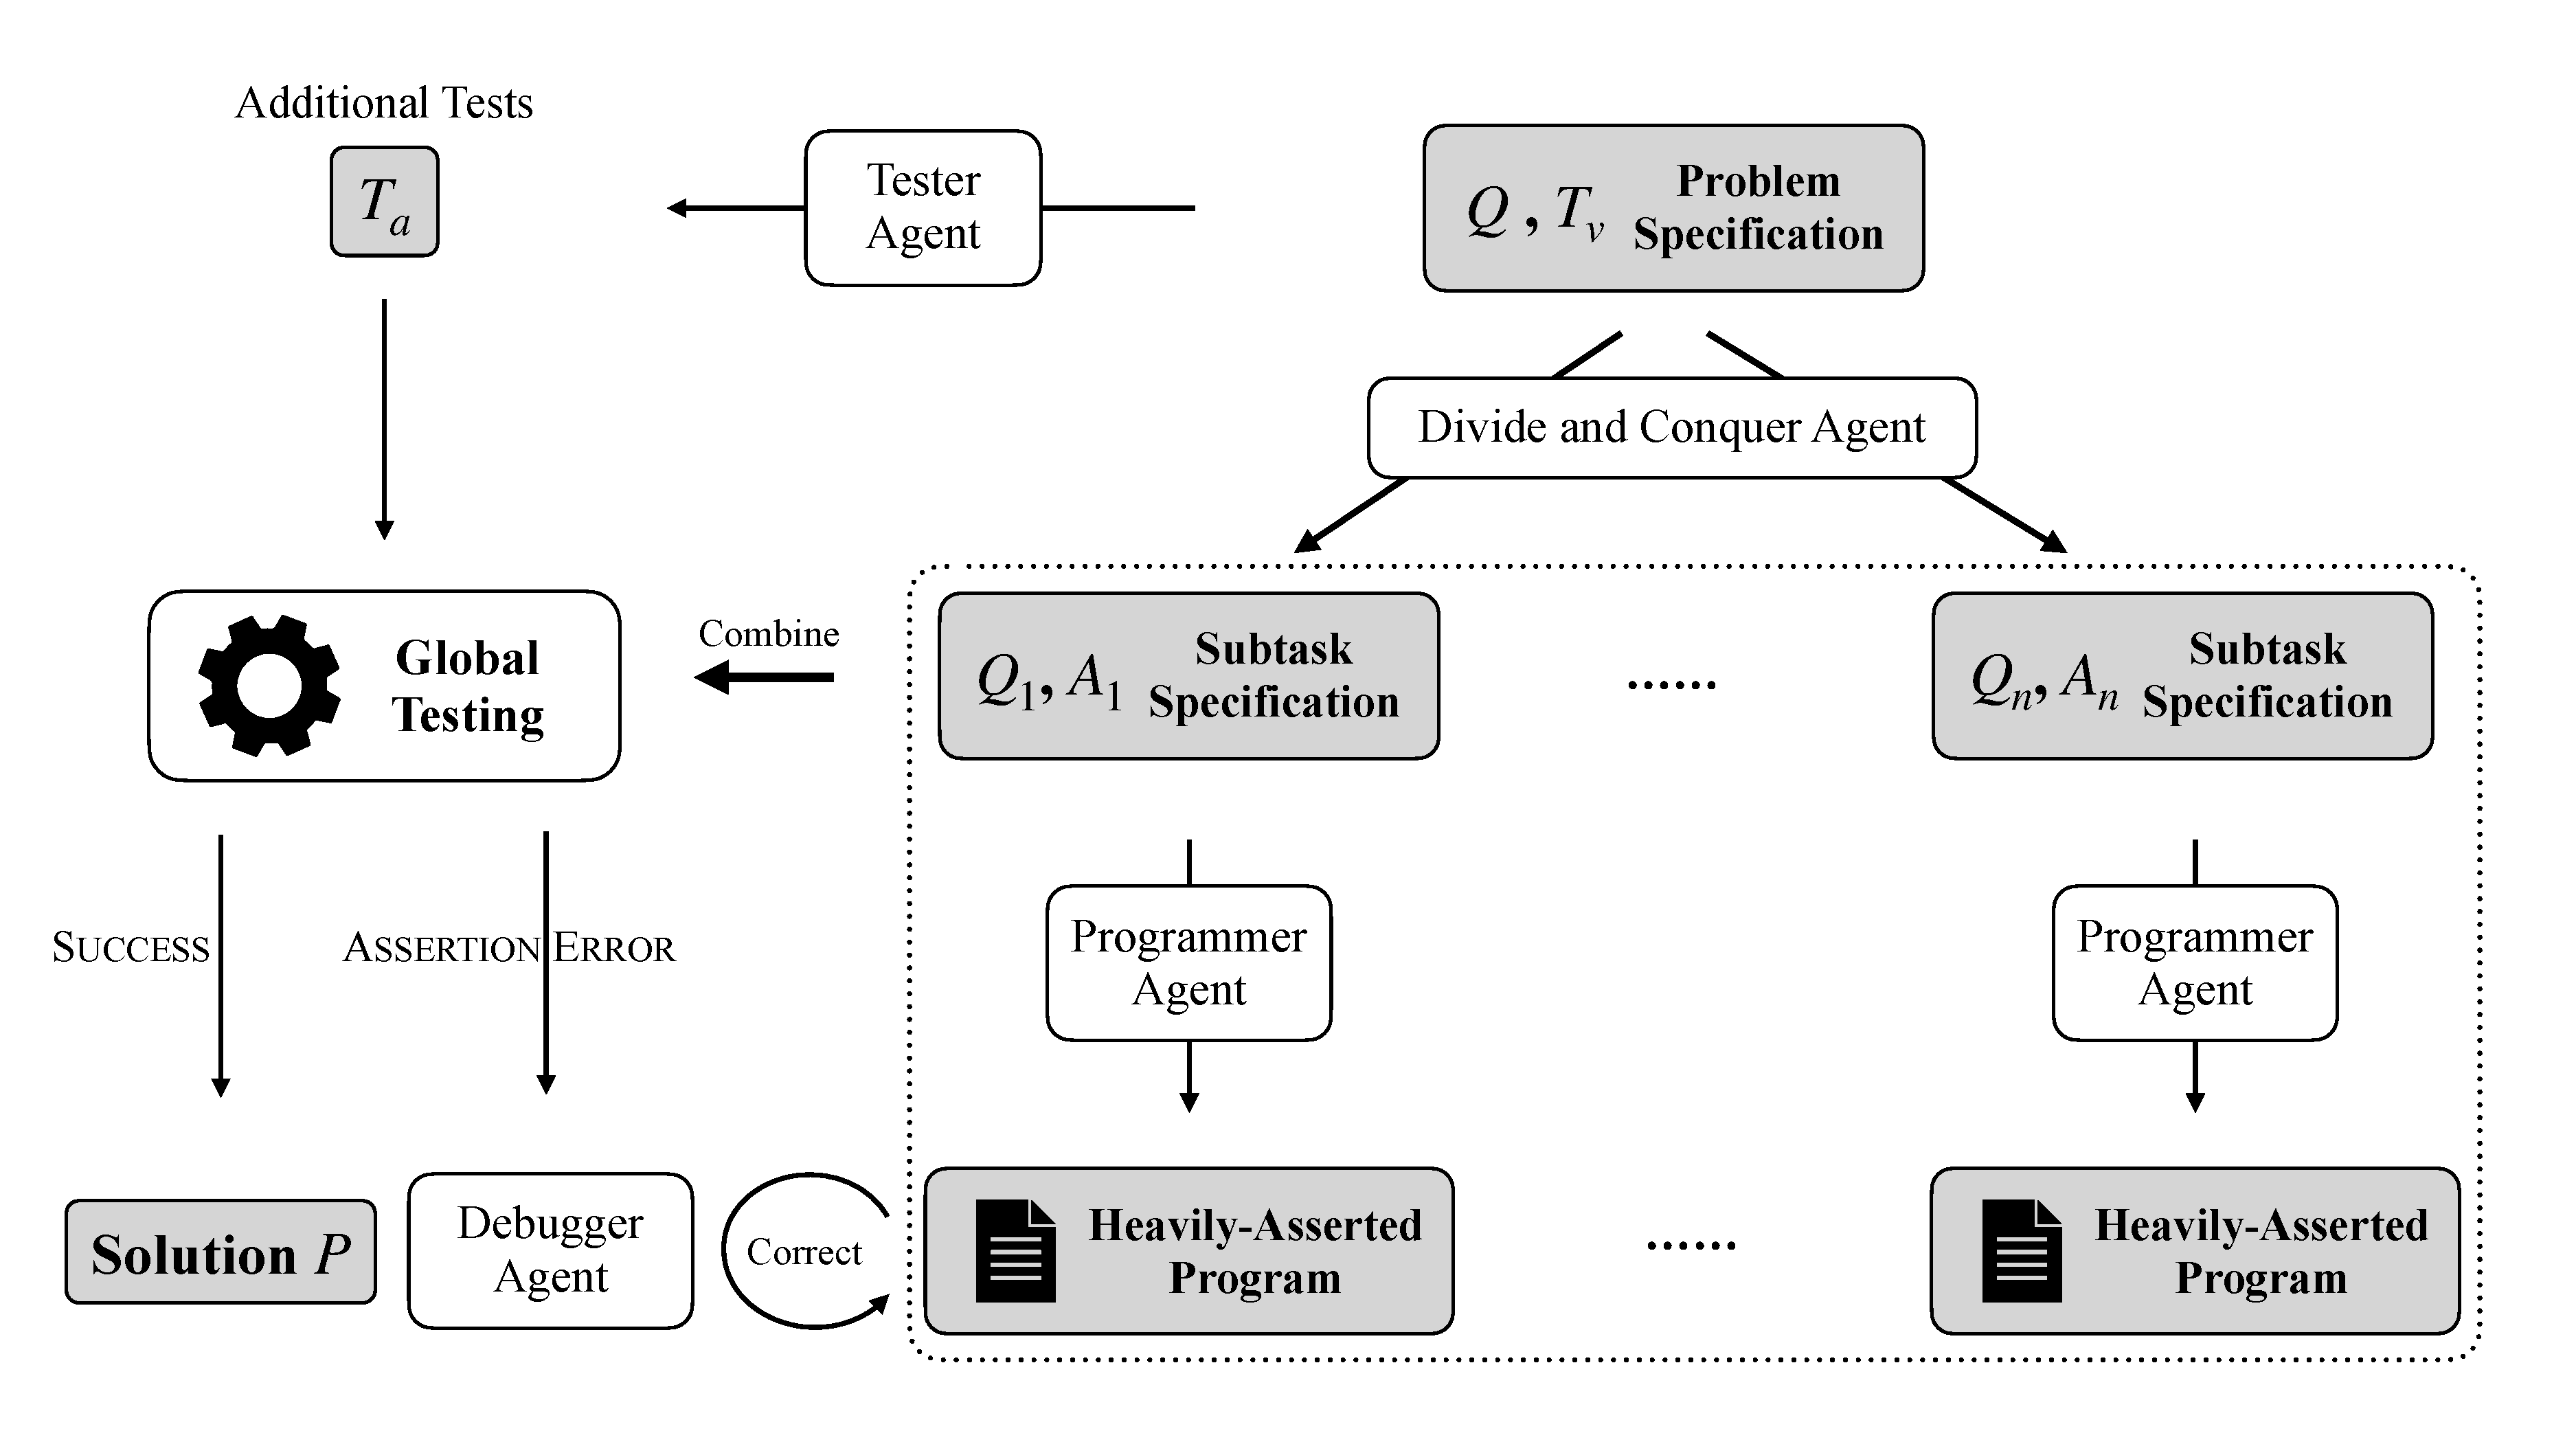
\includegraphics[width=\linewidth]{Architecture.pdf}
    \caption{Overview of the proposed assertion-based debugging framework.}
    \label{fig:overview}
\end{figure*}

Figure~\ref{fig:overview} illustrates an assertion-based debugging framework for large language models (LLMs), which follows a divide-and-conquer approach to problem-solving and debugging. The problem specification will be repeatedly decomposed into smaller subtasks specifications by a divide-and-conquer agent. Each subtask is represented as $(Q_i, A_i)$ where $Q_i$ is the natural language description of the subtask and $A_i$ is a set of assertions that the solution must satisfy. The divide-and-conquer agent will also generate codes to assemble all subprograms into a single unified program. Each subtask will then be assigned to a programmer agent, which generates a heavily-asserted program containing numerous assertions to detect potential errors. These individual programs are later combined into a complete solution using code generated by the divide-and-conquer agent.

While generating the individual programs, the tester agent concurrently generates hundreds of test cases to evaluate the correctness of the program. Once the combined program is generated, the global testing phase evaluates the program using predefined and additional test cases generated by the tester agent. If the program passes all tests, it is accepted as the final solution. Otherwise, if an assertion error is detected, a debugger agent steps in to correct the errors in the program, and the process iterates until a successful solution is reached. The debugger agents are able to navigate the program and identify the root cause of the assertion error, and then decide either to update the assertion or the code. This framework mimics expert debugging techniques by embedding assertions, systematically identifying issues, and refining solutions iteratively.

% It is worth noting that, the debugger agent, the tester agent and the programmer agents in the framework can work \textit{concurrently} without depending on the completion of each other. This parallel processing capability enhances the efficiency and scalability of the framework, enabling rapid debugging and solution generation for complex programming tasks. The framework's modular design allows for easy integration of additional agents or functionalities, making it adaptable to diverse programming scenarios.

\subsection{Prompt Design}

Since the proposed framework requires a large amount of assertions to generated by the programmer agent, the prompt used to guide the LLMs must be carefully designed to produces desired assertions. We must specify exactly what kind of assertions we want the LLMs to generate, and how to incorporate these assertions into the generated code. The prompt design should also consider the balance between the number of assertions and the complexity of the generated code, as an excessive number of assertions may lead to code bloat and performance degradation.

Here we list the important categories of assertions that we aim to specify in the prompt:

\begin{enumerate}
    \item \textbf{Input Assertions} specify the constraints that the input data must satisfy. These assertions are especially useful for checking the correctness of the combination program generated by the divide-and-conquer agent.
    \item \textbf{Output Assertions} specify the expected output of the program. A lot of engineering efforts need to put into those assertions, as they are the most important part of the program. Thus we force the model to generate such assertions, and recommand the model to create helper functions to check the output match the specialization exactly. For example, in a sorting algorithm, an output assertion may specify that the output list must be sorted in ascending order, which may involves a helper function \texttt{isSorted} to ensure that list is completely sorted.
    \item \textbf{Loop Invariants} can potentially help the model to understand the loop structure and the expected behavior of the loop without using information from long-distance context, and thus generate more accurate assertions. This would be more important in the future if we allow the model to interact with program verifiers.
\end{enumerate}

